\section{Simulations}\label{sec:simulations}

In this chapter, we will test the previously described MPC in a virtual environment. Throughout the simulations, the whole complexity of the humanoid will be condensed in a single point, representing its CoM.\\
The objective of this set of tests is to prove that, using the inputs provided by the MPC proposed by Peng et al. in \cite{peng_main_paper} and developed by us, a robot is able to reach a user-defined goal, while avoiding collisions with all the obstacles in the environment.\\
The hyperparameters used in the following simulations are summarized in Table \ref{table:sim_params}.

\begin{table}[h]
        \begin{tabular}{ |p{4cm}||p{4cm}| }
             \hline
             \multicolumn{2}{|c|}{Simulation Parameters} \\
             \hline
             \textbf{Parameter} & \textbf{Value}\\
             \hline
             $\alpha$   & 1.44 \\
             CoM height & 1 \si{\meter} \\
             Step duration ($T$) & 0.4 \si{\second} \\
             $l_{\max}$ & $0.1 \sqrt{3} \;\si{\meter}$ \\
             $\left( v_{x_{min}},\, v_{y_{min}} \right)$ & $\left( -0.1,\, 0.1 \right)$ \si{\meter\per\second}\\
             $\left( v_{x_{max}},\, v_{y_{max}} \right)$ & $\left( 0.8,\, 0.4 \right)$ \si{\meter\per\second}\\
             \hline
        \end{tabular}
    \centering
    \caption{The MPC and LIP parameters used for all the simulations in this chapter.}
    \label{table:sim_params}
\end{table}

\subsection{Simple Environment}\label{subsec:sim_simple_env}
The first simulation takes place in a basic environment: the humanoid is positioned at $(0,\,0)$ with orientation $\theta = 0$, and the goal position is $(5,\,5)$. In between, we placed 3 obstacles with a quasi-circular shape. The choice of approximating circles with polygons was made to comply with the CBF computation described in \ref{subsec:ldcbf}. The results are shown in Figures \ref{fig:sim1_evol} and \ref{fig:sim1_frames}.

By inspecting the plots, we see that, at the beginning of the simulation, a high turning velocity $\omega$ is commanded in order to make the robot point toward the goal. In the meantime, the MPC provides new footstep positions but, due to the maneuverability constraint, the high turning rate limits the velocity along the sagittal axis. Therefore, the robot is encouraged to move laterally, and the first inputs generate a large $v_y$ that induces a \textit{side-walking} motion.\\
Then, there is an overshoot in the plots of $\theta$ and $\omega$. This behavior derives from the large sampling time of the robot. To lighten the computational load, in our simulations, we set equal sampling times for the MPC and the humanoid. This means that every $T$ seconds a new footstep position and angular velocity are computed, and they are provided as input to the robot until new inputs are available, even though it could have a lower sampling time and, then, several different inputs could be commanded during $T$. Therefore, the $\omega$ needed to point to the goal is provided as input and executed for $T$ seconds. But, during that interval, the robot misses the right orientation and continues rotating. Hence, a new turning velocity is commanded in the opposite direction, and the sagittal axis is successfully aligned with the goal.\\
At this point, the robot moves forward to the goal, the orientation is kept constant, and the positional error decreases smoothly. Nevertheless, there is some chattering in the $v_y$ plot. This is a regular behavior: at the end of each step, the humanoid changes the stance foot by \textit{falling} on the opposite side, and it results in the lateral velocity changing sign.\\
Around the second 35 of the simulation (4th and 5th frames of Figure \ref{fig:sim1_frames}), the humanoid approaches one of the obstacles. It is unable to go forward, as this would lead the CoM into the circle. To keep the robot in the safe area defined by the LDCBF, the new MPC solution makes the humanoid move laterally. Thus, it can successfully avoid the obstacle. In this case, \textit{side walking} occurs because the precomputed value of $\omega$ only aims at aligning the sagittal axis of the robot with the goal, and, once it is achieved, the turning rate is kept constant. Consequently, the humanoid can only escape the obstacle while facing the goal. This movement explains the minor variations in the position error and translational velocity plots around the second 35.\\
The humanoid can, then, realign itself (producing a minimal oscillation in the $\theta$ and $\omega$ plots) and continue navigating to the goal, which it ultimately reaches successfully.

\begin{figure}[H]
    \centering
    \begin{subfigure}{0.45\linewidth}
        \centering
        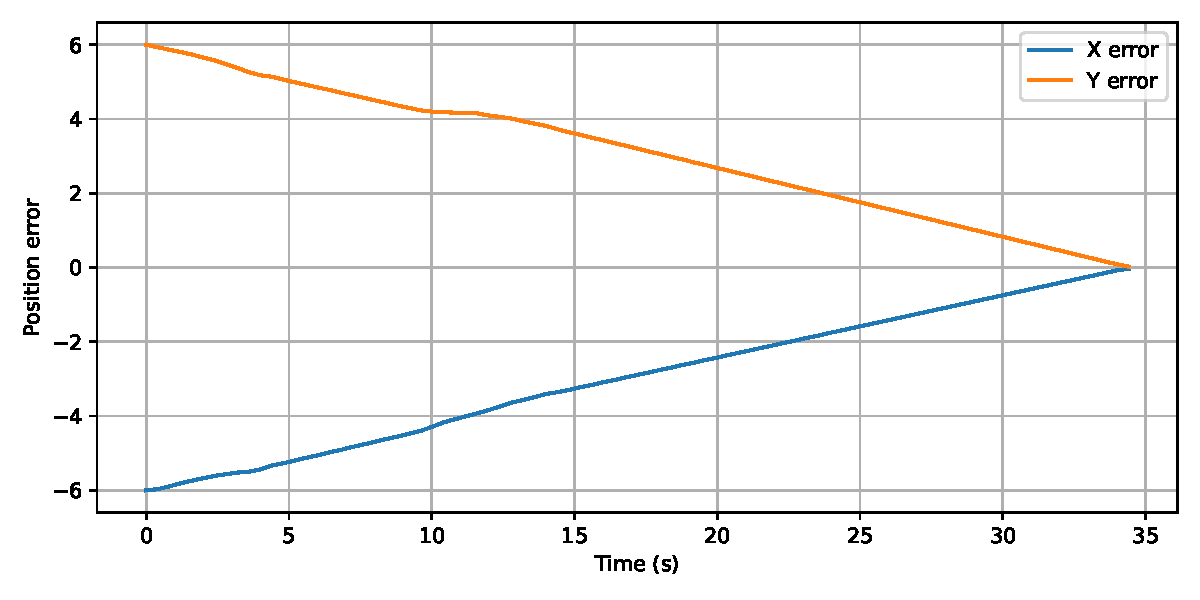
\includegraphics[width=\linewidth]{figures/Simulations/sim1circles/evolution_0.pdf}
    \end{subfigure}
    \begin{subfigure}{0.45\linewidth}
        \centering
        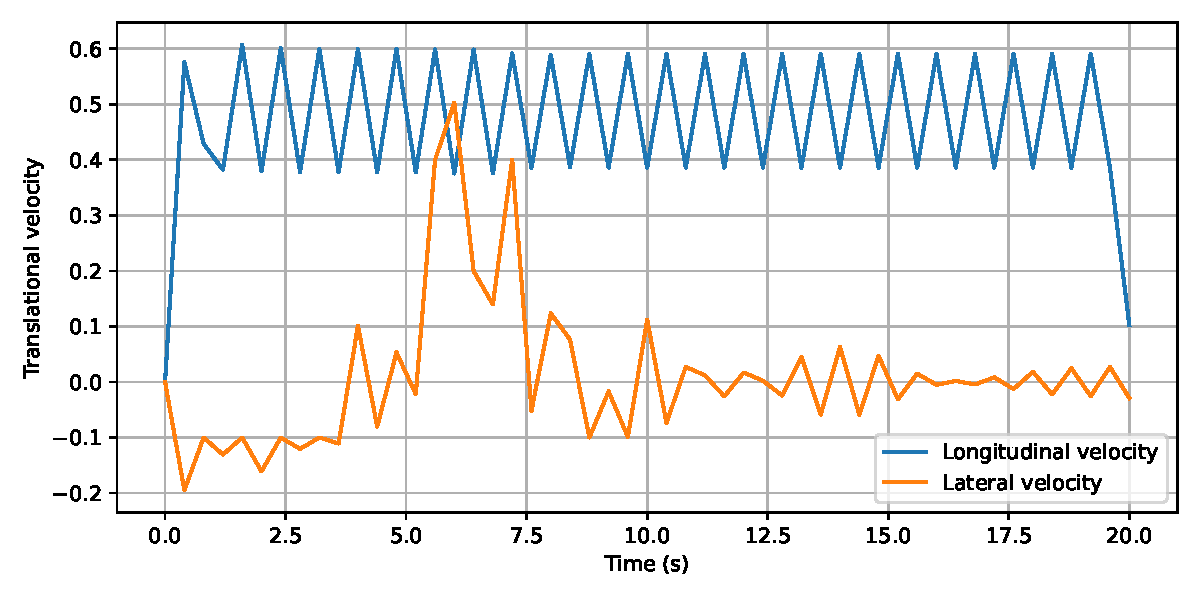
\includegraphics[width=\linewidth]{figures/Simulations/sim1circles/evolution_1.pdf}
    \end{subfigure}
    \hfill
    \begin{subfigure}{0.45\linewidth}
        \centering
        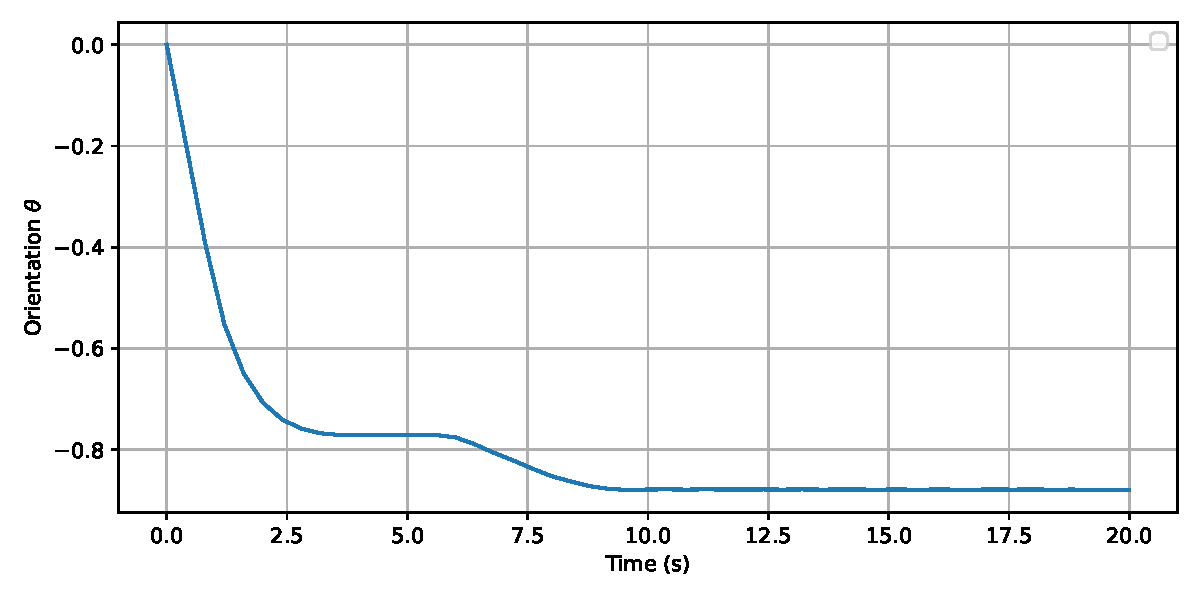
\includegraphics[width=\linewidth]{figures/Simulations/sim1circles/evolution_2.pdf}
    \end{subfigure}
    \begin{subfigure}{0.45\linewidth}
        \centering
        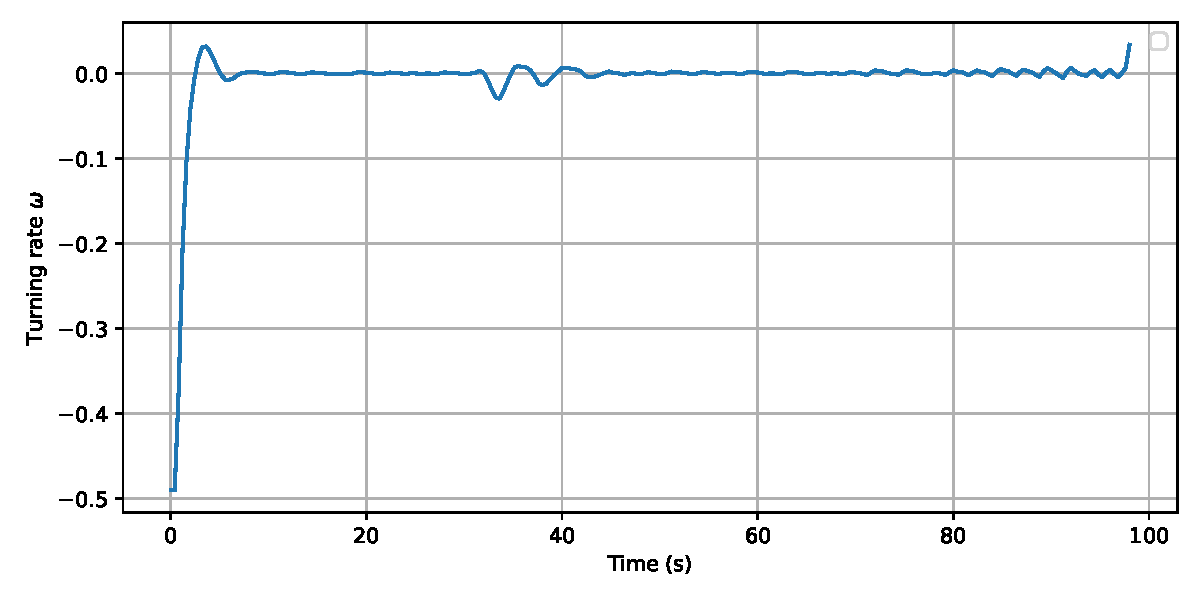
\includegraphics[width=\linewidth]{figures/Simulations/sim1circles/evolution_3.pdf}
    \end{subfigure}
    \caption{These figures depict the evolution of the humanoid's state and the input throughout the simulation. The top-left plot shows the error between the CoM and the goal position, while the top-right represents the translational velocities along the x- and y-axis. The bottom left and right plots show the theta and omega evolution, respectively. All the quantities are expressed in the global RF.}
    \label{fig:sim1_evol}
\end{figure}

\begin{figure}[H]
    \centering
    % First row
    \begin{subfigure}{0.20\textwidth}
        \centering
        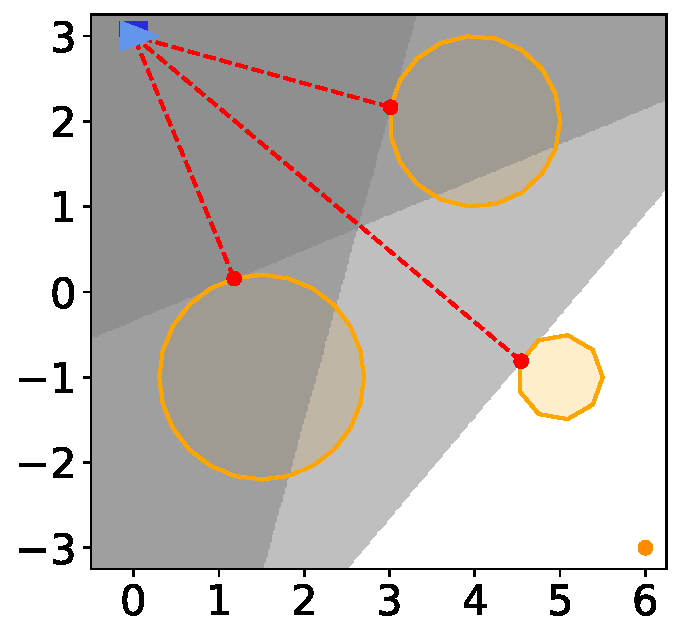
\includegraphics[width=\textwidth]{figures/Simulations/sim1circles/frame_0.pdf}
    \end{subfigure}%
    \hfill
    \begin{subfigure}{0.20\textwidth}
        \centering
        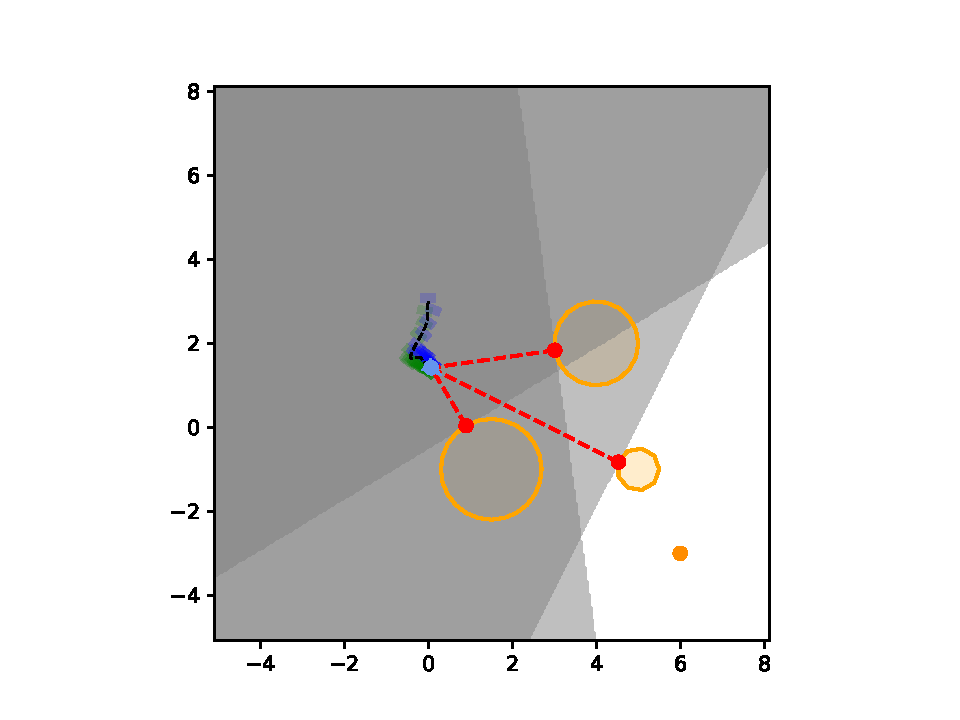
\includegraphics[width=\textwidth]{figures/Simulations/sim1circles/frame_1.pdf}
    \end{subfigure}%
    \hfill
    \begin{subfigure}{0.20\textwidth}
        \centering
        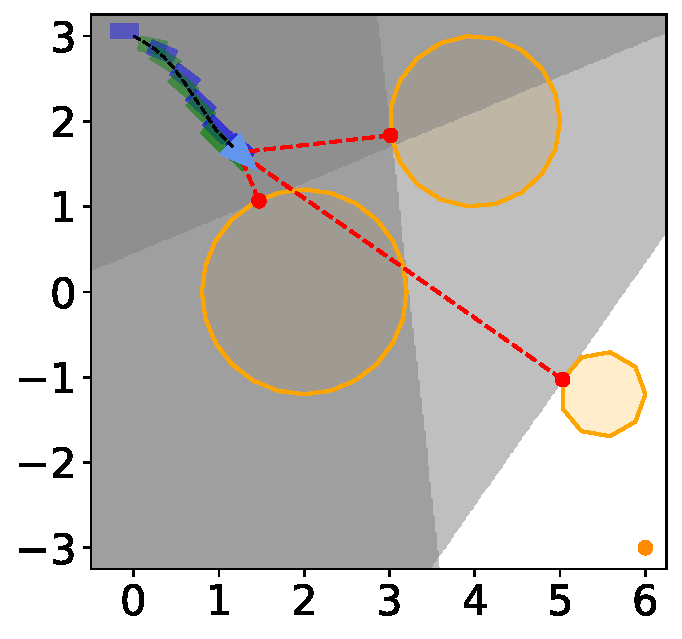
\includegraphics[width=\textwidth]{figures/Simulations/sim1circles/frame_2.pdf}
    \end{subfigure}%
    \hfill
    \begin{subfigure}{0.20\textwidth}
        \centering
        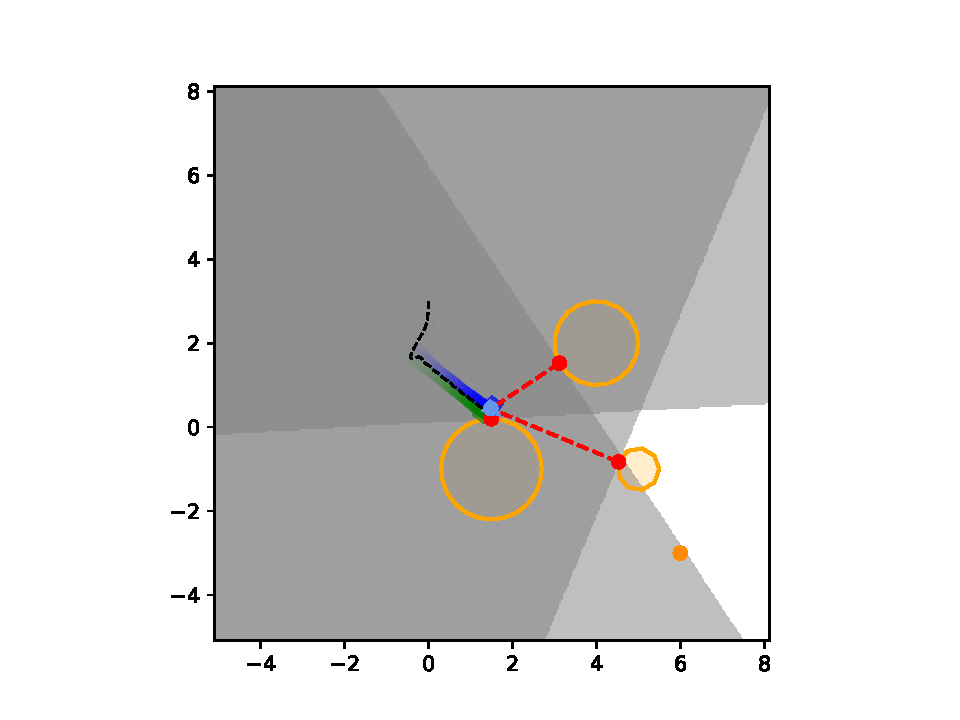
\includegraphics[width=\textwidth]{figures/Simulations/sim1circles/frame_3.pdf}
    \end{subfigure}%
    \hfill
    \begin{subfigure}{0.20\textwidth}
        \centering
        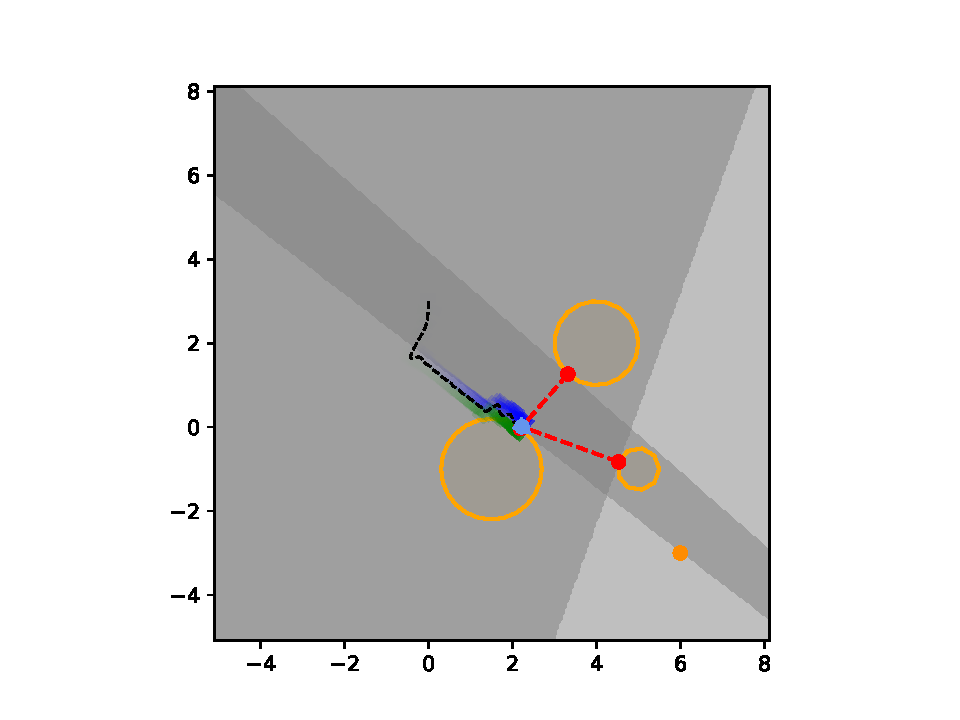
\includegraphics[width=\textwidth]{figures/Simulations/sim1circles/frame_4.pdf}
    \end{subfigure}
    
    % Second row
    \begin{subfigure}{0.20\textwidth}
        \centering
        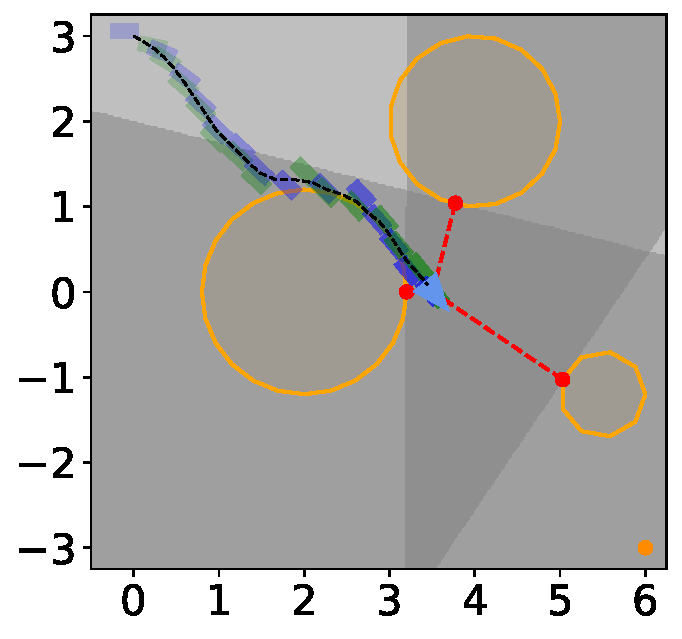
\includegraphics[width=\textwidth]{figures/Simulations/sim1circles/frame_5.pdf}
    \end{subfigure}%
    \hfill
    \begin{subfigure}{0.20\textwidth}
        \centering
        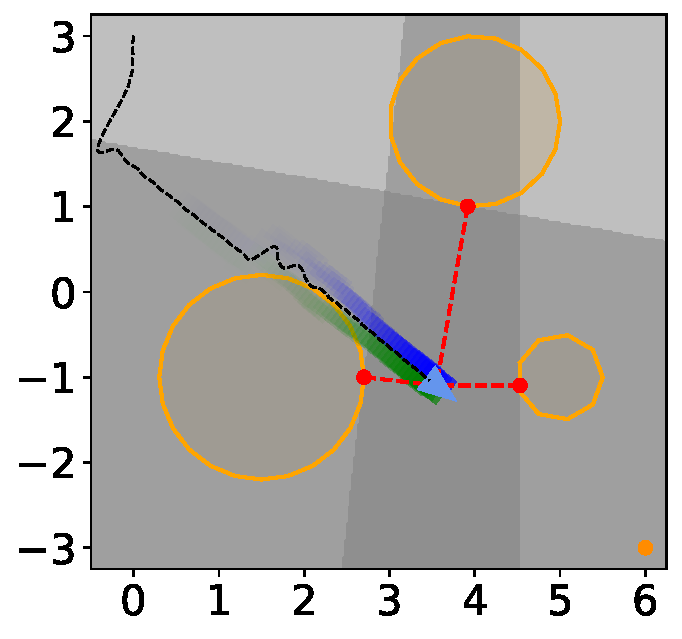
\includegraphics[width=\textwidth]{figures/Simulations/sim1circles/frame_6.pdf}
    \end{subfigure}%
    \hfill
    \begin{subfigure}{0.20\textwidth}
        \centering
        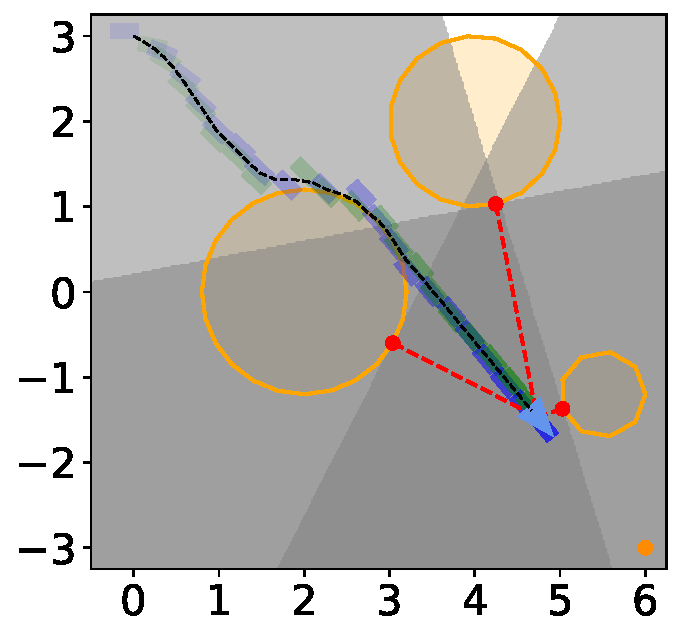
\includegraphics[width=\textwidth]{figures/Simulations/sim1circles/frame_7.pdf}
    \end{subfigure}%
    \hfill
    \begin{subfigure}{0.20\textwidth}
        \centering
        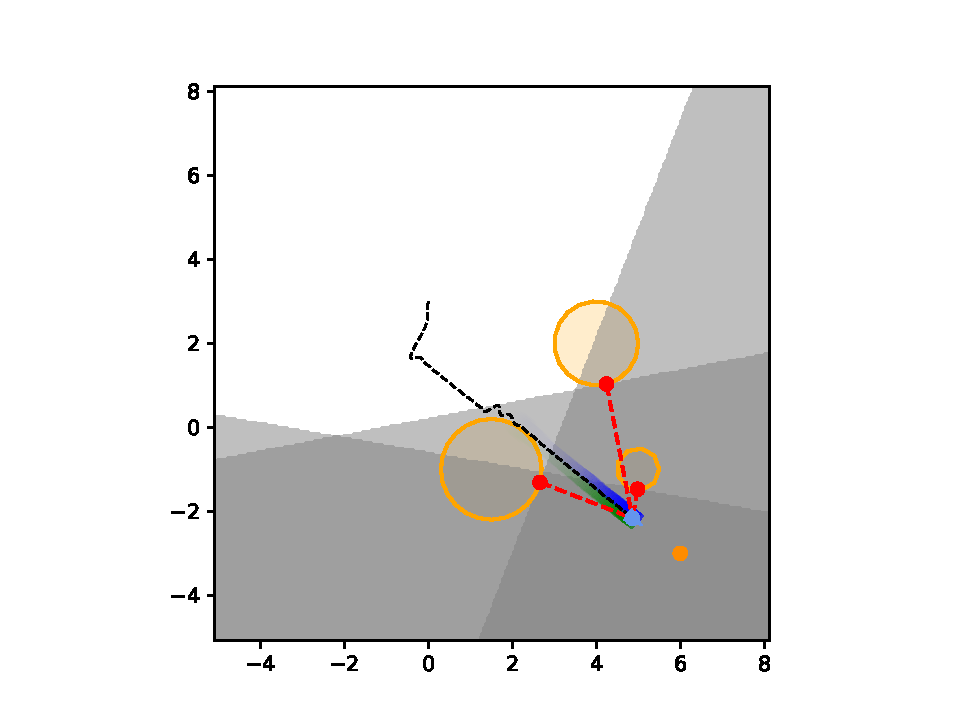
\includegraphics[width=\textwidth]{figures/Simulations/sim1circles/frame_8.pdf}
    \end{subfigure}%
    \hfill
    \begin{subfigure}{0.20\textwidth}
        \centering
        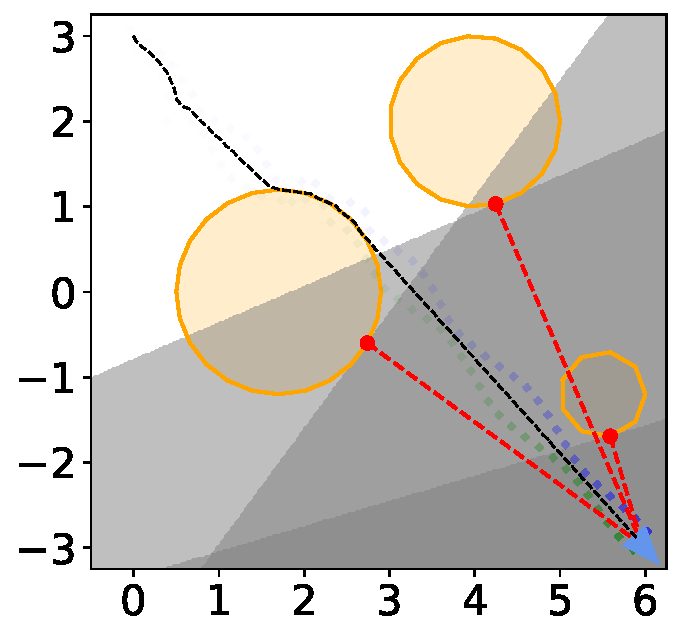
\includegraphics[width=\textwidth]{figures/Simulations/sim1circles/frame_9.pdf}
    \end{subfigure}
    
    \caption[short]{This sequence of frames illustrates the robot's trajectory to the goal. Obstacles are represented with orange shapes. The humanoid is represented by an isosceles triangle whose sagittal axis is aligned with the robot's. Green rectangles mark right footsteps, while blue rectangles mark left ones. Each frame shows the vectors $\eta$ and $c$ along with the safe area associated with each obstacle. The darkest region represents the intersection of these semi-planes, which is the overall safe area.}
    \label{fig:sim1_frames}
\end{figure}

\subsubsection{Simulation employing our LDCBF}
From an accurate analysis of the previous simulation's frames, it can be observed that, despite the robot accomplishing the mission of reaching the goal while satisfying all the constraints, when it gets very close to the obstacles, its feet overlap with the obstacles. This occurs due to the LDCBF defined by Peng et al., which only ensures that the CoM never collides with the obstacles. However, this strategy produces a path that is impractical for the full-body motion of the humanoid (as already pointed out in \ref{subsec:ldcbf_variant}). Therefore, we proposed our variant of their LDCBF, and in Figures \ref{fig:sim1_delta_evol} and \ref{fig:sim1_delta_frames} we show the results of the simulation that constraints the MPC with the LDCBF defined at \ref{eq:ldcbf_variant}, setting $\delta=0.3$.

From the plots, we notice that the robot reaches the boundary of the safe area -- no longer coincident with the obstacle's edge -- earlier than the previous simulation, and it reorients itself with the modality exposed before. The same situation arises around the second 70 of the simulation, when a turning velocity is commanded to keep a distance $\delta$ from the last obstacle.

The simulation frames in Figure \ref{fig:sim1_delta_frames} reveal that the humanoid's footsteps never intersect the obstacles. Subsequently, the LDCBF contributed to designing a motion plan suitable for the humanoid in real-world conditions.

\begin{figure}[H]
    \centering
    \begin{subfigure}{0.45\linewidth}
        \centering
        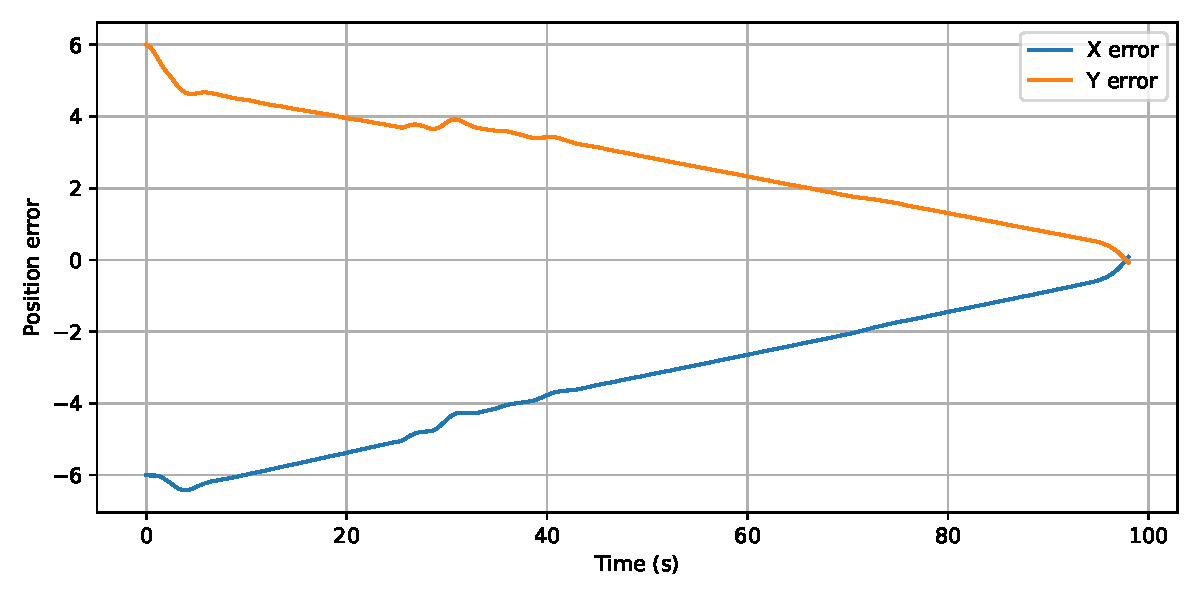
\includegraphics[width=\linewidth]{figures/Simulations/sim1circles_delta/evolution_0.pdf}
    \end{subfigure}
    \begin{subfigure}{0.45\linewidth}
        \centering
        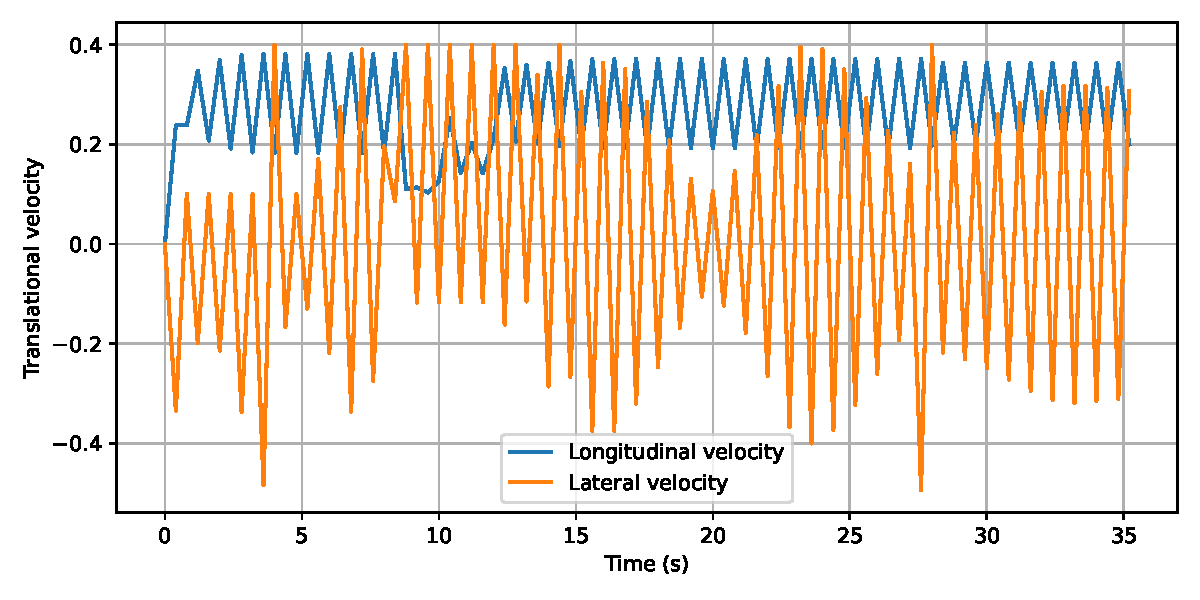
\includegraphics[width=\linewidth]{figures/Simulations/sim1circles_delta/evolution_1.pdf}
    \end{subfigure}
    \hfill
    \begin{subfigure}{0.45\linewidth}
        \centering
        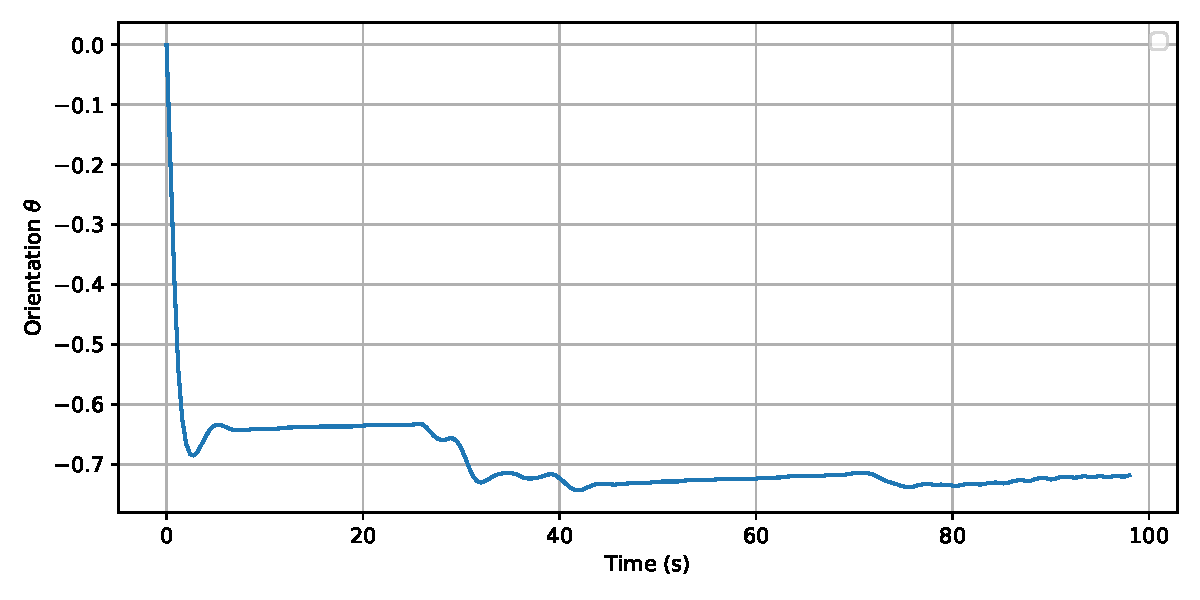
\includegraphics[width=\linewidth]{figures/Simulations/sim1circles_delta/evolution_2.pdf}
    \end{subfigure}
    \begin{subfigure}{0.45\linewidth}
        \centering
        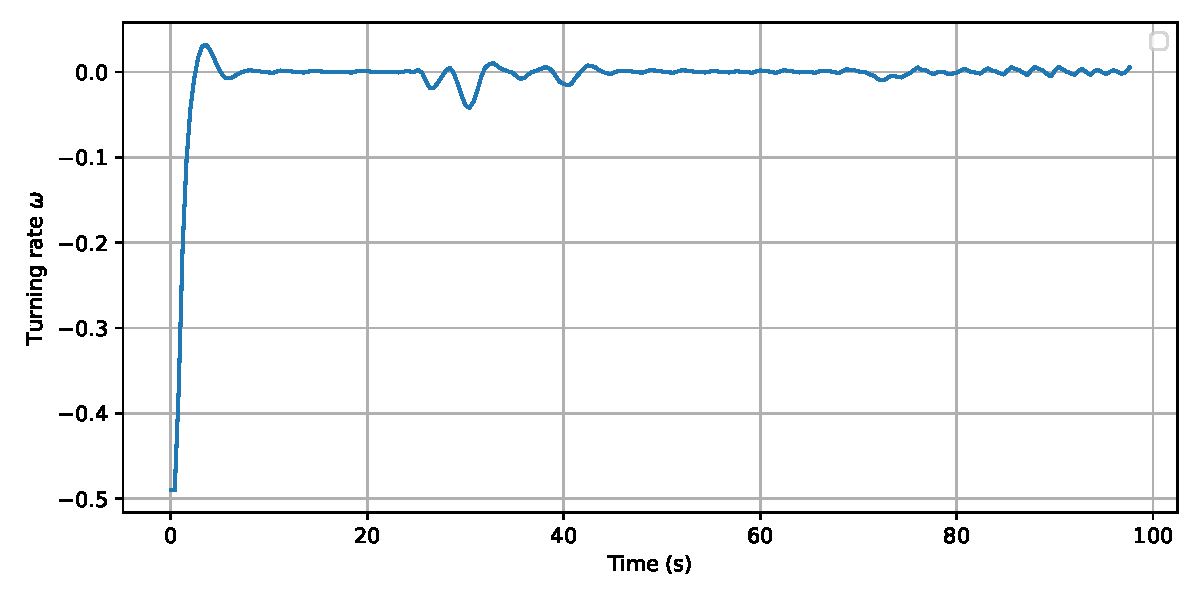
\includegraphics[width=\linewidth]{figures/Simulations/sim1circles_delta/evolution_3.pdf}
    \end{subfigure}
    \caption{These figures depict the evolution of the humanoid's state and the input throughout the simulation in the base environment employing our LDCBF. The top-left plot shows the error between the CoM and the goal position, while the top-right represents the translational velocities along the x- and y-axis. The bottom left and right plots show the theta and omega evolution, respectively. All the quantities are expressed in the global RF.}
    \label{fig:sim1_delta_evol}
\end{figure}

\begin{figure}[H]
    \centering
    % First row
    \begin{subfigure}{0.20\textwidth}
        \centering
        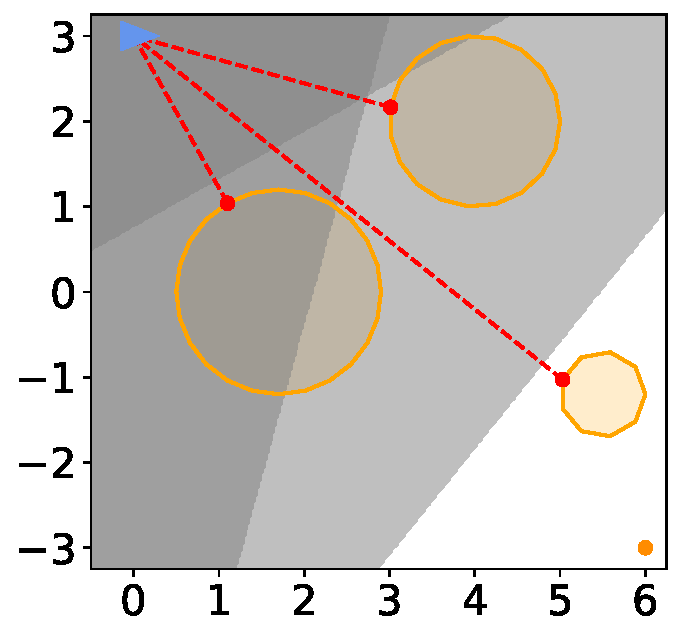
\includegraphics[width=\textwidth]{figures/Simulations/sim1circles_delta/frame_0.pdf}
    \end{subfigure}%
    \hfill
    \begin{subfigure}{0.20\textwidth}
        \centering
        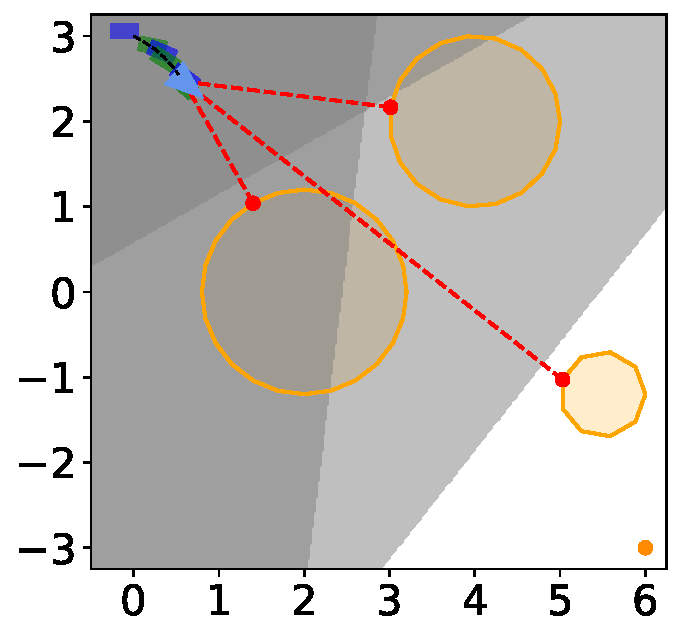
\includegraphics[width=\textwidth]{figures/Simulations/sim1circles_delta/frame_1.pdf}
    \end{subfigure}%
    \hfill
    \begin{subfigure}{0.20\textwidth}
        \centering
        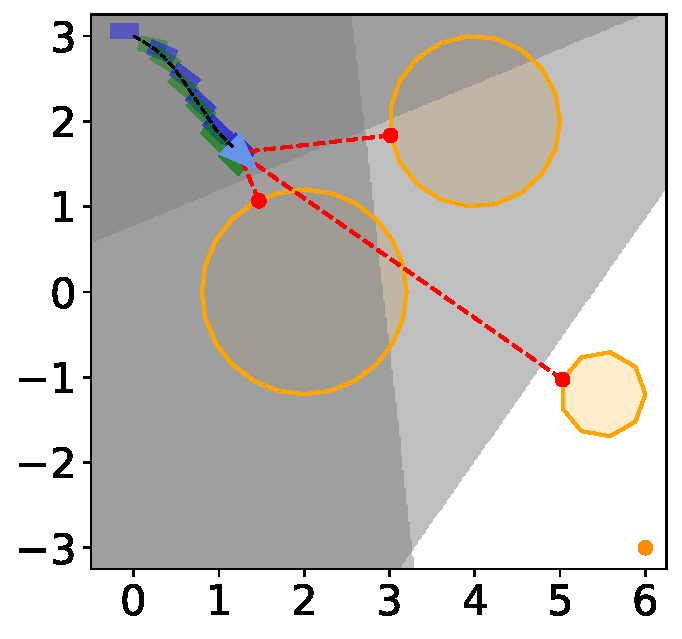
\includegraphics[width=\textwidth]{figures/Simulations/sim1circles_delta/frame_2.pdf}
    \end{subfigure}%
    \hfill
    \begin{subfigure}{0.20\textwidth}
        \centering
        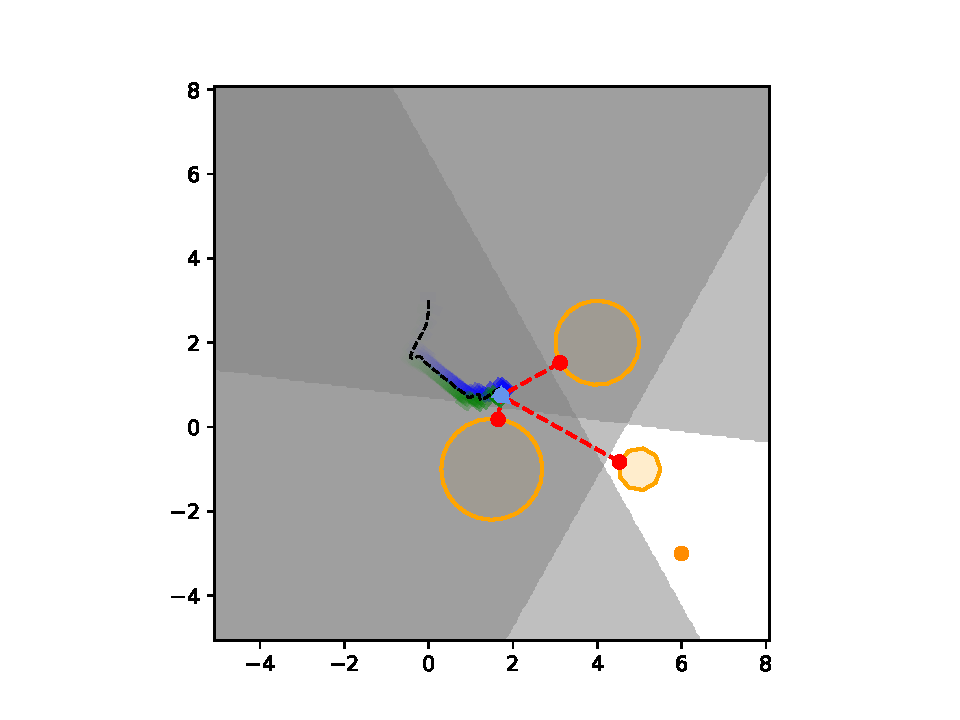
\includegraphics[width=\textwidth]{figures/Simulations/sim1circles_delta/frame_3.pdf}
    \end{subfigure}%
    \hfill
    \begin{subfigure}{0.20\textwidth}
        \centering
        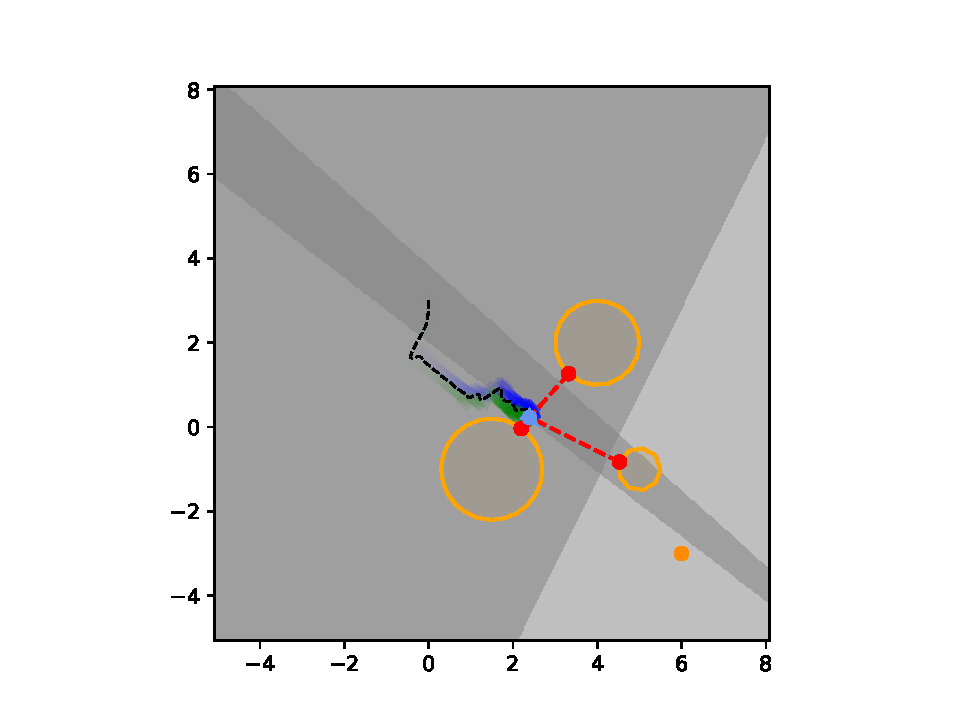
\includegraphics[width=\textwidth]{figures/Simulations/sim1circles_delta/frame_4.pdf}
    \end{subfigure}
    
    % Second row
    \begin{subfigure}{0.20\textwidth}
        \centering
        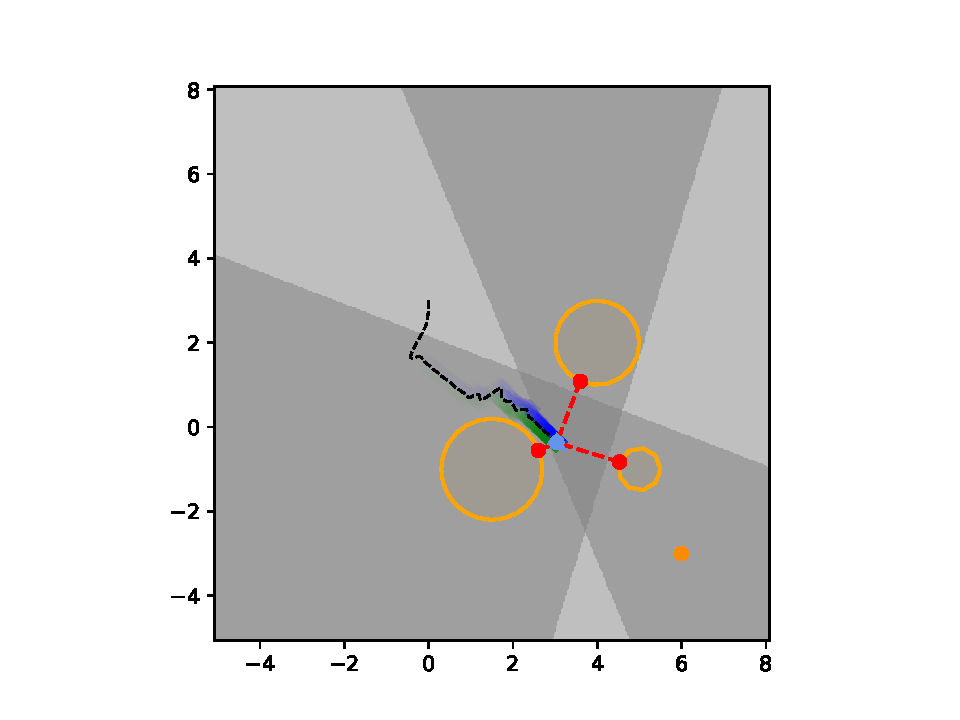
\includegraphics[width=\textwidth]{figures/Simulations/sim1circles_delta/frame_5.pdf}
    \end{subfigure}%
    \hfill
    \begin{subfigure}{0.20\textwidth}
        \centering
        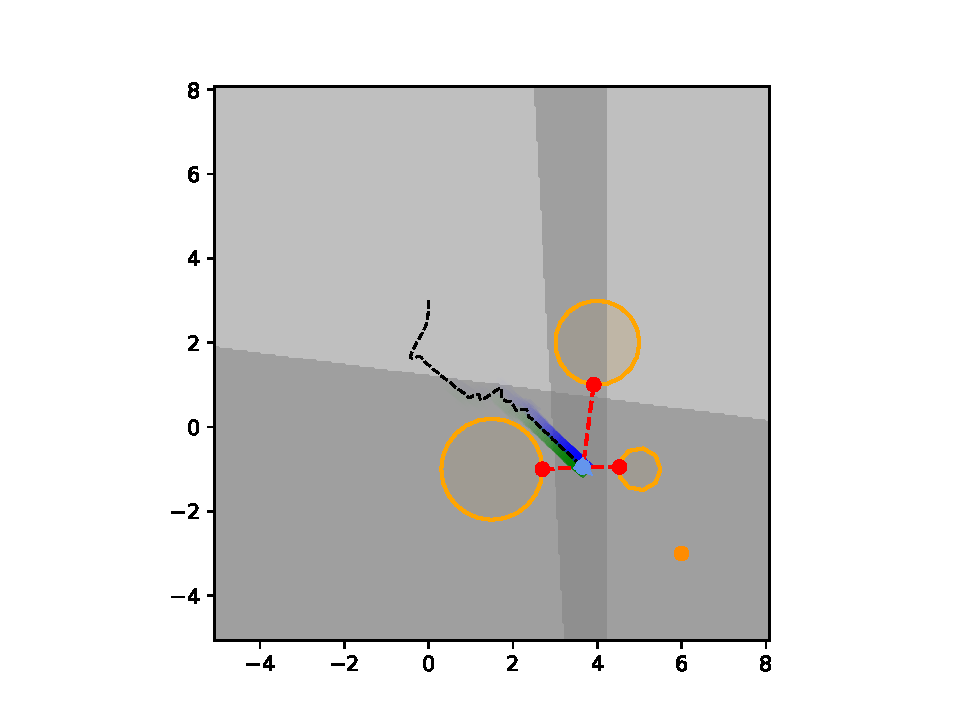
\includegraphics[width=\textwidth]{figures/Simulations/sim1circles_delta/frame_6.pdf}
    \end{subfigure}%
    \hfill
    \begin{subfigure}{0.20\textwidth}
        \centering
        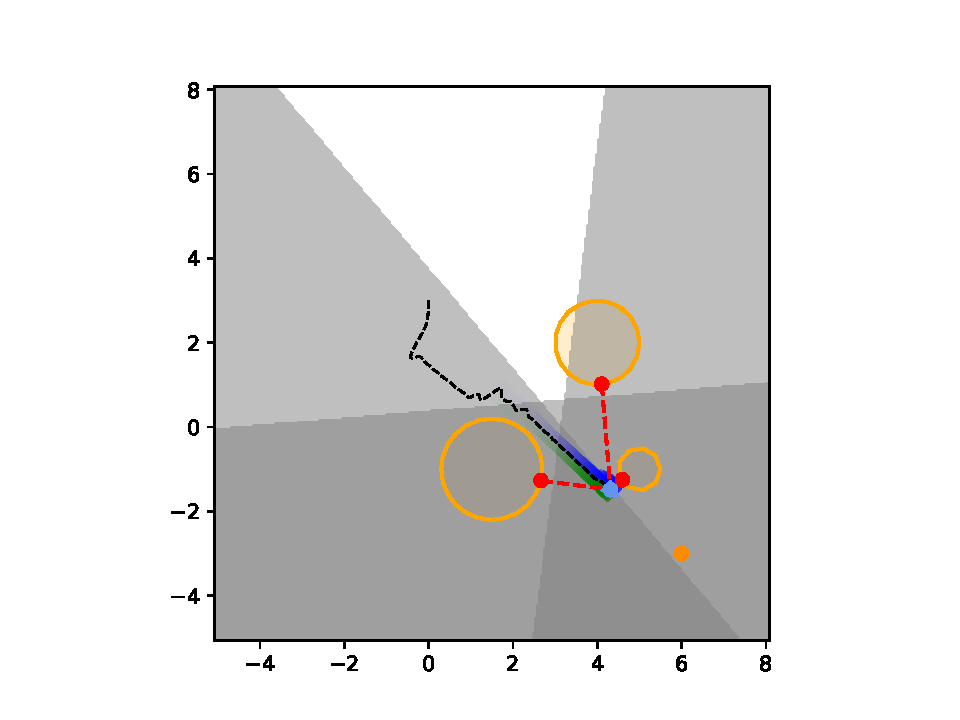
\includegraphics[width=\textwidth]{figures/Simulations/sim1circles_delta/frame_7.pdf}
    \end{subfigure}%
    \hfill
    \begin{subfigure}{0.20\textwidth}
        \centering
        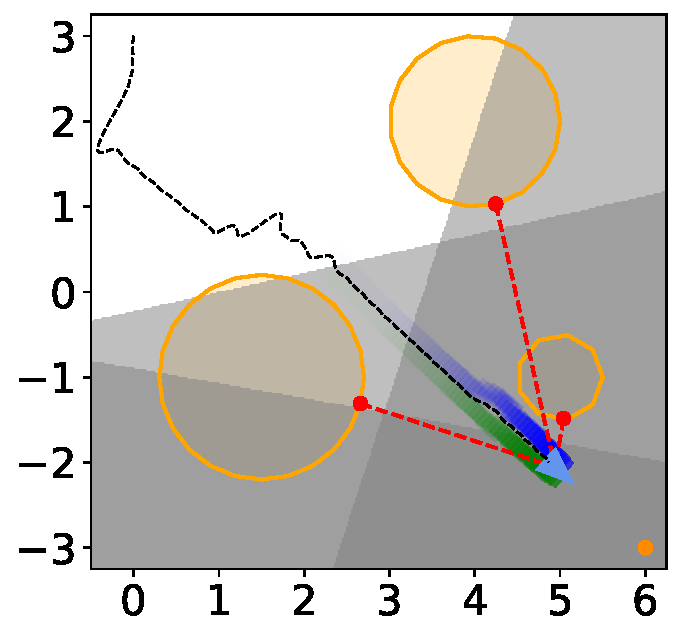
\includegraphics[width=\textwidth]{figures/Simulations/sim1circles_delta/frame_8.pdf}
    \end{subfigure}%
    \hfill
    \begin{subfigure}{0.20\textwidth}
        \centering
        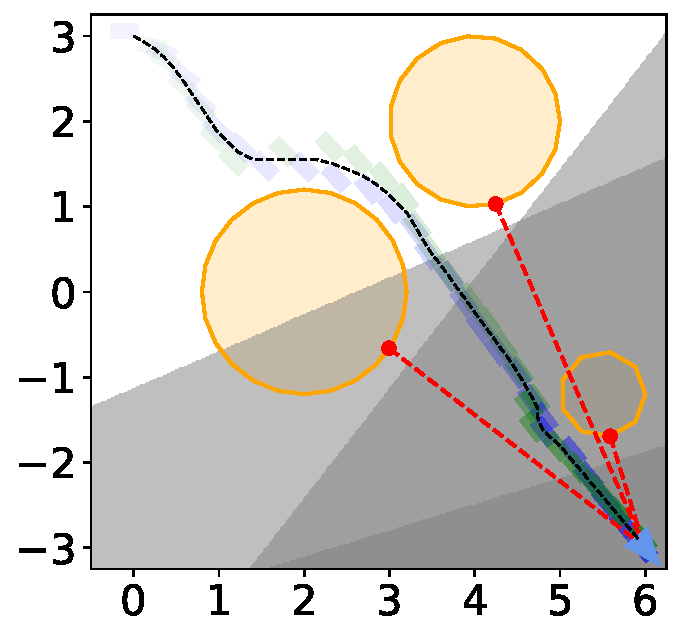
\includegraphics[width=\textwidth]{figures/Simulations/sim1circles_delta/frame_9.pdf}
    \end{subfigure}
    
    \caption[short]{This sequence of frames illustrates the robot's trajectory to the goal for the simulation in the base environment employing our LDCBF. With this modification, the darkest region (i.e., the overall safe area) never touches the obstacles boundaries, but is always at a user-defined distance $\delta$.}
    \label{fig:sim1_delta_frames}
\end{figure}